\def\busslide{
  \begin{frame}{Visão lógica do sistema de barramentos}{}
    \begin{figure}[h]
      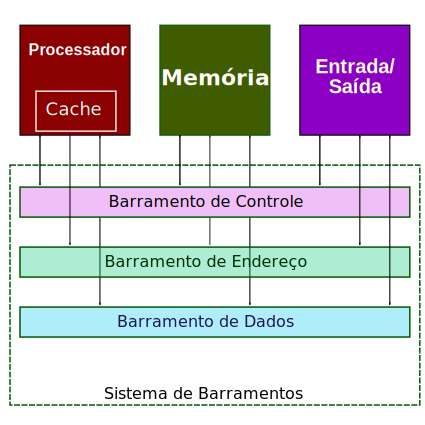
\includegraphics[scale=.625]{\imgdir/zfig-bus-logic}
    \end{figure}
  \end{frame}
}

\lecture{Entrada/Saída (E/S)}{io}
\lecturetitle{\insertlecture}{\course}
\frame{\maketitle}

\busslide

\begin{frame}{Conexões}{processador, memória e dispositivos de E/S}{}\small
  {\only<2->{\color{gray}} \alert{Transações de E/S: } sequência de
    operações processador-memória\footnote{\tiny Com exceção de alguns
      dispositivos como placa de vídeo.}  e dispositivo de E/S sobre a
    interconexão, que inclui uma requisição e pode incluir uma
    resposta, e também pode
    transmitir dados. \\
  } \pause\bigskip

  {\only<1,3->{\color{gray}} \alert{Barramento síncrono:} inclui um
    relógio (\emph{clock}) que controla as linhas de transmissão e um
    protocolo de comunicação comandado pelo \emph{clock}.  }
  \pause\bigskip

  {\only<1-2>{\color{gray}} \alert{Interconexão asssíncrona:}
    Usa um protocolo \emph{handshaking} (aperto de mão) ao invés
    do \emph{clock} para coordenar a transação. Pode acomodar uma
    grande variedade de dispositivos de diferentes velocidades.
  }

\end{frame}

\begin{frame}{Comandos para os dispositivos de E/S}{}
  {\only<2->{\color{gray}} \alert{E/S mapeada na memória:} esquema
    de E/S em que partes do espaço de endereçamento são atribuídos a
    dispositivos de E/S. Leituras e Escritas para estes endereços são
    interpretados como comandos para os dispositivos de E/S.
  }
  \pause\bigskip

  {\only<1>{\color{gray}}
    \alert{Instrução de E/S:} instrução dedicada que é usada para dar um comando para
    um dispositivo de E/S e que especifica o número do dispositivo e a palavra do comando
    (ou local da palavra do comando na memória).
  }
\end{frame}

\begin{frame}{Comunicação com o processador}

  {\only<2->{\color{gray}} \alert{\emph{Polling} (sondagem):}
    processo do processador periodicamente checar o status de um dispositivo de
    E/S para determinar a necessidade de servir este dispositivo.    
  }  
  \pause\bigskip

  {\only<1>{\color{gray}}
    \alert{Interrupção de E/S:} esquema de E/S que emprega interrupções para
    indicar ao processador que um dispositivo de E/S precisa de atenção.
    Na interrupção, cada dispositivo tem uma identificação e recebe um nível
    de prioridade para ser atendido.
  }  
\end{frame}

\begin{frame}{Transferência de dados}{dispositivo e memória}
  {\only<2->{\color{gray}} Normalmente o processador é utilizado pelos
    dispositivos de E/S para transferir dados para ou da memória.
  }
  \pause\bigskip
  
  {\only<1>{\color{gray}}
    \alert{Acesso direto à memória (DMA--\emph{direct memory access}):}
    um mecanismo que fornece ao controlador do dispositivo com habilidade
    de transferir dados diretamente para ou da memória sem o envolvimento
    do processador.
  }
  
\end{frame}

\begin{frame}{Referência}{}
\begin{thebibliography}{3}
\bibitem{patterson2008}[Patterson, 2008]
  {David A. Patterson; John L. Hennessy},
  \newblock                {Computer Organization and Design},
  \newblock    {Morgan Kaufmann Publisher, 2008},
\end{thebibliography}
\end{frame}

%%%%%%%%%%%%%%%%%%%%%%%%%%%%%%%% BUS

\lecture{E/S: Barramentos}{bus}
\lecturetitle{\insertlecture}{\course}

\frame{\titlepage}

\section{Introdução}

\begin{frame}{Arquitetura do barramento}{Barrramento}
  \begin{itemize}
  \item Caminho de dados (datavia);
    \item Caminhos independentes;
    \item Possibilidade de expansão;
    \item Diferença entre os barramentos está na:
      \begin{itemize}
      \item Quantidade de bits transmitidos por vez;
      \item Frequência de operação.
      \end{itemize}
  \end{itemize}
  
  
\end{frame}


\busslide

\def\thetitle{Barramento ISA}
\section{\thetitle}
\begin{frame}{\thetitle}
  \begin{columns}
    \begin{column}{.575\textwidth}
      \footnotesize
      \begin{itemize}
      \item ISA -- {\em Industry Standard Architecture};
      \item Desenvolvido pela IBM em 1981;
      \item Sistema inicial com 8 bits, extendido para 16 bits em 1983;
      \item Sem suporte a {\em plug and play}: 
         \begin{itemize}
           \item 8 bits, 7 MHz, 7 MB/s;
             \item 16 bits: 14 MHz, 14 MB/s;
         \item Acesso direto à memória;
        \item Ajuste ``manual'' do identificado das requisições de
          interrupção (IRQ).
        \end{itemize}
      \end{itemize}
    \end{column}
    \begin{column}{.475\textwidth}
      \begin{center}
        {\tiny Fonte: \url{http://en.wikipedia.org/wiki/Industry_Standard_Architecture}}\\
        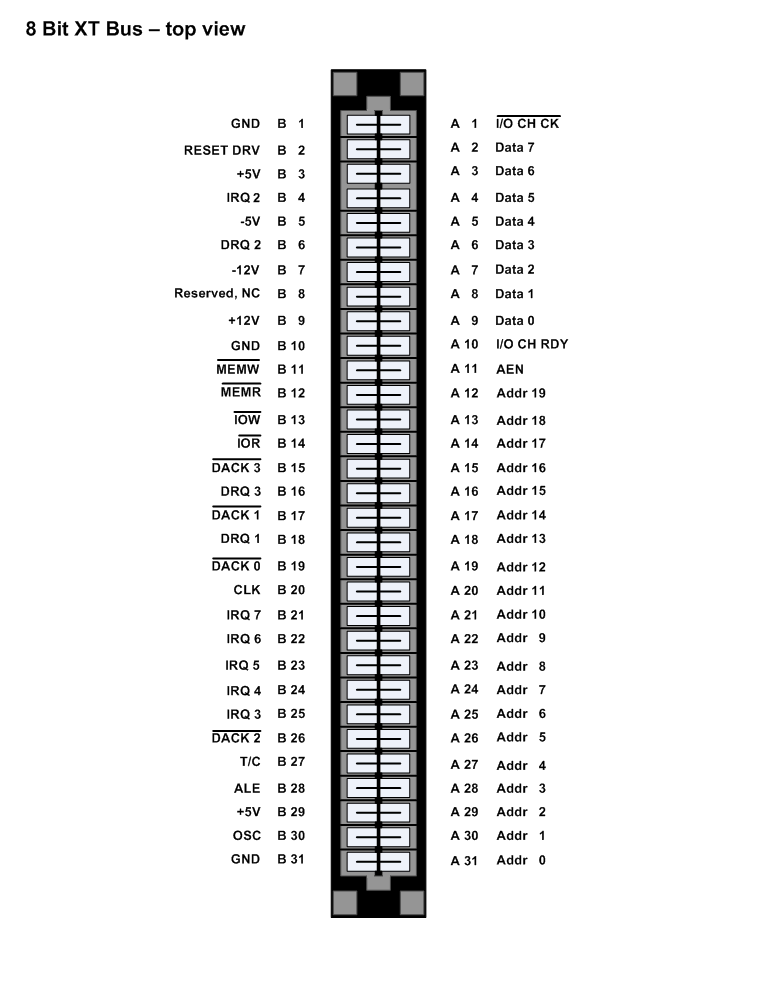
\includegraphics[scale=.325]{\imgdir/zfig-bus-isa_xt_pins.png}
      \end{center}  
    \end{column}
  \end{columns}
\end{frame}

\def\thetitle{Barramento PCI}
\section{\thetitle}

\begin{frame}{\thetitle}
  \framesubtitle{{\em Peripheral Component Interconnect}}
  
  \begin{itemize}
  \item Desenvolvido pela Intel em 1993;
  \item Banda: 32 ou 64 bits;
  \item Velocidade de transmissão: 133/266/533 MB/s.
  \end{itemize}
\begin{center}
  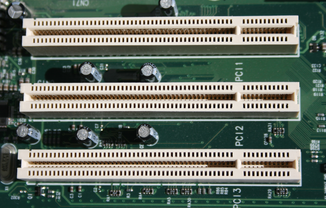
\includegraphics[scale=.5]{\imgdir/zfig-pci_slot.png}\\
  {\small {\em Slot} PCI}
\end{center}
\end{frame}

\begin{frame}{Barramentos PCI e ISA}
\begin{figure}[h]
  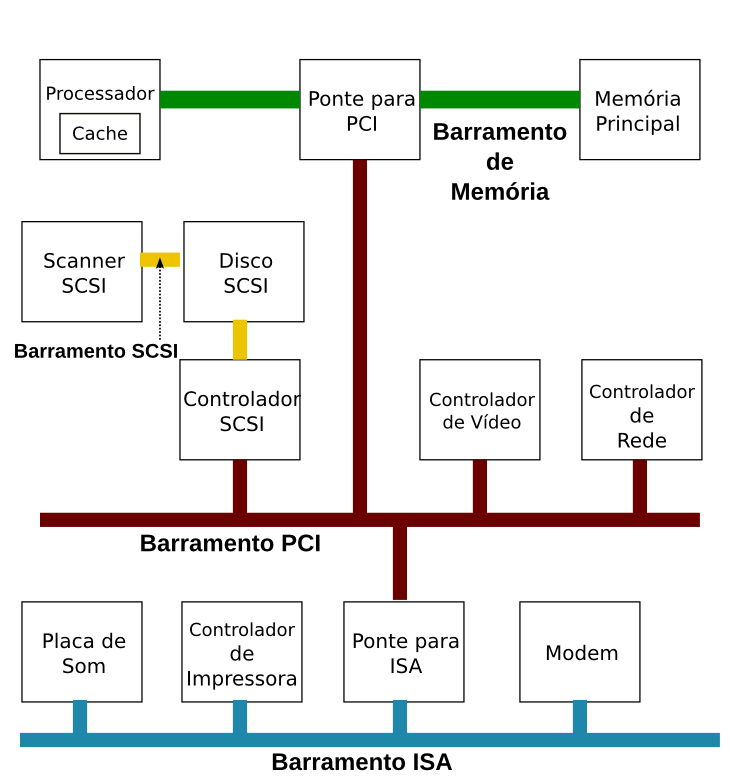
\includegraphics[scale=.325]{\imgdir/zfig-bus-pci_isa}
\end{figure}
\end{frame}

\def\thetitle{Barramentos atuais}
\section{\thetitle}

\begin{frame}{\thetitle}{AGP (Acellerated Graphics Port), PCI-Express}
\footnotesize
  Transmissão de dados convergindo para a serial ao invés de
  paralela. Motivos:
  \begin{itemize}
  \item Menor quantidade de fios, reduzindo a interferência eletromagnética;
  \item Transmissão em {\em full-duplex} ao invés de {\em half-duplex};
  \item Na transmissão paralela os bits são transmitidos ao mesmo
    tempo, mas podem não chegar ao mesmo tempo gerando exceções;
  \item Apesar transmitir menos dados por vez, a velocidade de
    transmissão é maior que a paralela.
  \end{itemize}
  
  Houve necessidade do aumento da transmissão de dados no barramento
  principalmente devido às exigências das aplicações gráficas.\\
\begin{center}
  \begin{tabular}{|c|c|}\hline
    Tecnologia & Velocidade de transmissão (MB/s)  \\\hline
    ISA & 14 \\
    PCI & 533 \\
    AGP 8x & 2.133 \\
    PCI-EXpress x32 & 8.000 \\\hline
  \end{tabular}
\end{center}
\end{frame}

% Arquitetura de Computadores: Prof. Mario F. G. Boaratti
% Fonte: http://docslide.com.br/documents/3-barramentos.html
% Sinais de controle:  φ = relógio. 
% - ENDERECO: sinais de enderecamento. 
% - DADOS: dados a transferir. 
% - ~MREQ: requisicao de referencia a memoria. Ativo em baixo. 
% - ~RD: ativo = leitura, inativo = escrita. Ativo em baixo. 
% - ~WAIT: sinaliza estado de espera  ate que a memoria consiga atender a requisicao. Ativo em  baixo. 
% - Operacao:  A operacao e disparada transicao positiva do relogio em T1. 
% - O processador  coloca o endereco, que ele quer ler, 
% na linha de endereço durante
% o meio ciclo alto de T1. Para representar que o endereço não é um
% valor único ele é representado por duas linhas que se cruzam no
% instante que o endereço é enviado (área branca).  Após
% estabilização do endereço, disparado pela transição, o
% processador ativa MREQ para indicar que é a memória que está
% sendo acessada e RD para indicar que é uma leitura.  No
% início de T2, a memória ativa WAIT, sinalizando que não tem
% condições de fornecer o dado neste ciclo, uma vez que a memória
% leva 15ηs, após o endereço estar estável, para responder. Esta
% ação inserirá estados de espera no barramento até que a memória
% conclua e desative WAIT.  Na transição positiva de T3, a
% memória desativa WAIT, sinalizando que terá os dados disponíveis
% neste ciclo.
\section{Barramento Síncrono}

\def\ymax{24} % 6 * 4 \/ 3 * 8
\def\deltachange{0.8} % "tempo" p/ o sinal mudar o valor 1/10 Ti, como
                      % T1=T2=T3=8, deltaT=0.8
\def\xzero{0cm}
\def\yzero{1cm}
\def\deltax{2cm}
\def\deltay{1cm}

\def\delay{0.15cm}
\def\protox{-2*\delay} % start before the coordinates
% DADOS
\def\drawdata#1{
  \def\xbase{#1}
  \def\datay{4*\deltay-\deltay/2}
  \pgfpathmoveto{\pgfpoint{\protox}{\datay}}
  \pgfpathlineto{\pgfpoint{\xbase}{\datay}}
  \pgfpathlineto{\pgfpoint{\xbase+\deltax}{\datay}}
  \pgfpathlineto{\pgfpoint{\xbase+\deltax}{\datay+\deltay}}
  \pgfpathlineto{\pgfpoint{\xbase}{\datay+\deltay}}
  \pgfpathlineto{\pgfpoint{\protox}{\datay+\deltay}}
  \pgfsetfillcolor{red}
  \pgfusepath{fill,stroke}
}

\def\drawaddress#1{
  \def\xlimit{#1}
  \def\ady{5*\deltay} % start of ADDRESS in y
  \foreach \e in {0,1} {
    \pgfpathmoveto{\pgfpoint{\xlimit}{\ady+\e*\deltay}}
    \pgfpathlineto{\pgfpoint{\deltax/2+\delay}{\ady+\e*\deltay}}
    \pgfpathlineto{\pgfpoint{\deltax/2}{\ady+0.5*\deltay}}
  } % foreach e in ...
  \pgfsetfillcolor{white}
  \pgfusepath{stroke}
} % drawaddress

\def\drawcycle#1#2{
  \def\cx{#1}
  \def\cycleindex{#2}
  \def\cy{6.5*\deltay}
  \def\rcx{\cx*\deltax}
  \def\timearrow{} %default

  \ifnum\cx=0
  \pgfpathmoveto{\pgfpoint{\cx+\protox}{\cy}}
  \pgfpathlineto{\pgfpoint{\cx-\delay}{\cy}}
  \pgfpathlineto{\pgfpoint{\cx}{\cy+\deltay/2}}
  \pgfusepath{stroke}
  \draw (\cx,-\deltay) -- (\cx,10*\deltay);
  \fi
  
  \ifodd\cx
  % multiplier to control curve behaviour
  \def\mul{0} \def\scale{9}%
  \def\timearrow{\draw[<->] (\rcx-\deltax,8.5) -- (\rcx+\deltax,8.5);
                 \node[anchor=center] at (\rcx,9)%
                 {\scriptsize T$_{\cycleindex}$};}% end \def\timearrow
  \else
  \def\mul{1} \def\scale{8}
  \fi
  
  \draw (\rcx+\deltax,\mul-1) -- (\rcx+\deltax,\scale*\deltay);
  \pgfpathmoveto{\pgfpoint{\rcx}{\cy+\deltay/2}}
  \pgfpathlineto{\pgfpoint{\rcx+\delay}{\cy+\mul*\deltay}}
  \pgfpathlineto{\pgfpoint{\rcx+\deltax-\delay}{\cy+\mul*\deltay}}
  \pgfpathlineto{\pgfpoint{\rcx+\deltax}{\cy+\deltay/2}}
  \pgfusepath{stroke}
  \timearrow

  \ifnum\cx=5
  \draw (\rcx+\deltax,-\deltay) -- (\rcx+\deltax,10*\deltay);
  \pgfpathmoveto{\pgfpoint{\rcx+\deltax}{\cy+\deltay/2}}
  \pgfpathlineto{\pgfpoint{\rcx+\deltax+\delay}{\cy+\deltay}}
  \pgfpathlineto{\pgfpoint{\rcx+\deltax-\protox}{\cy+\deltay}}
  \pgfusepath{stroke}
  \fi
  
}
 
\def\fsignal#1{{\scriptsize $#1$}}
\def\arrowlabel#1{{\tiny #1}}
\def\expandedlabelpos{(1.5*\deltax,10.75*\deltay)}
\def\emphrange#1#2#3{
  \def\xstart{#1}
  \def\ystart{#2}
  \def\xend{#3}
  % yend is fixed at 10.25*\deltay
  \draw[draw=yellow,fill=yellow,fill opacity=0.6] (\xstart,\ystart)
  rectangle (\xend,10.25*\deltay); 
}
\begin{frame}
\frametitle{Temporização em barramento síncrono}

\begin{tikzpicture}[scale=0.6,signal/.style={thick},
  expandedlabel/.style={shape=rectangle callout,fill=yellow!60,overlay}]
  %\draw[help lines] (0cm,0cm) grid (6*\deltax,8*\deltay);
 
  \only<1->{
    
    \draw[signal] (\protox,\yzero) node[left] {\fsignal{\overline{WAIT}}} -- 
    (\xzero,\yzero) -- (\deltax,\yzero);
    
    \def\rdy{\yzero+\deltay}
     \draw[signal] (\protox,\rdy) node[left] {\fsignal{\overline{RD}}} -- 
     (\xzero,\rdy) --  (\deltax,\rdy);
    
     \def\mreqy{\rdy+\deltay}
     \draw[signal] (\protox,\mreqy) node[left] {\fsignal{\overline{MREQ}}} --
     (\xzero,\mreqy) -- (\deltax,\mreqy);
     
     \def\waity{\mreqy+\deltay}
     
     % DADOS
     \node at (-0.75*\deltax,4*\deltay) {\fsignal{DADOS}};
     \only<1>{\drawdata{\xzero}}

     % ENDERECO
     \node[anchor=east] at (-\delay,5.5*\deltay) {\fsignal{ENDERE\text{\it \c{C}}O}};
     \def\ady{3.5*\deltay+1.5*\deltay} % start of ADDRESS in y
     \pgfpathmoveto{\pgfpoint{\protox}{\ady}}
     \pgfpathlineto{\pgfpoint{\deltax/2-\delay}{\ady}}
     \pgfpathlineto{\pgfpoint{\deltax/2}{\ady+\deltay/2}}
     \pgfpathlineto{\pgfpoint{\deltax/2-\delay}{\ady+\deltay}}
     \pgfpathlineto{\pgfpoint{\protox}{\ady+\deltay}}
     \pgfsetfillcolor{red}
     \pgfusepath{fill,stroke}

     \only<1>{\drawaddress{\deltax}} % address ja vem com a ponta
     
     % CYCLE
     \node at (-0.25*\deltax,6.5*\deltay) {\fsignal{\Phi}};
     \drawcycle{0}{1}

     % 1a cota
     \draw[dashed] (\deltax/2,\mreqy-\deltay/2) -- (0.5*\deltax,6.5*\deltay);

     % Tad
     \draw[<->] (0,6.25*\deltay) -- (\deltax/2,6.25*\deltay);
     \node (Tad) at (\deltax/4,6.5*\deltay) {\arrowlabel{T$_{AD}$}};
       
       \only<1>{
         \node[anchor=center,expandedlabel,callout absolute
         pointer={(Tad) ++(0.25*\deltax,0)}] at \expandedlabelpos {\arrowlabel{T$_{AD}$
             - Atraso de sa\'ida do endere\c{c}o}};
         \emphrange{0}{6.5*\deltay}{\deltax/2}
         % \node[expandedlabel,callout absolute pointer={(Tad)}] at
        % (\deltax,-2*\deltay) {\arrowlabel{T$_{ML}$ -- Endere\c{c}o
        %   est\'avel antes de MREQ}};
       }
       
   } % only<1>...

   \only<1-4>{\node at (\deltax,-\deltay) {\scriptsize Tempo $\longrightarrow$};}
   
   \only<2->{
     \draw[signal] (\xzero,\yzero) ++(\deltax,0) 
     -- (2*\deltax-\delay,\yzero) 
     -- (2*\deltax,\yzero-\deltay/4);
     
     \draw[signal] (\xzero+\deltax,\rdy) 
     -- (1.25*\deltax-\delay,\rdy)
     -- (1.25*\deltax,\rdy-\deltay/4)
     -- (1.25*\deltax+\delay,\rdy-\deltay/2)
     -- (2*\deltax,\rdy-\deltay/2);

     % 2a cota
     \draw[dashed] (1.25*\deltax,\rdy-4*\delay) -- % delay here is only
     (1.25*\deltax,\rdy+\deltay+2*\delay); % reused, no meaning at all
    
     % Tml
     \draw[<->] (0.5*\deltax,\mreqy-2*\delay) -- (1.25*\deltax,\mreqy-2*\delay);
     \node (Tml) at (0.75*\deltax,\mreqy-4*\delay) {\arrowlabel{T$_{ML}$}};
     
     \only<2>{
       \emphrange{0.5*\deltax}{\mreqy-4*\delay+4*\delay}{1.25*\deltax};
       \node[anchor=north west,expandedlabel,callout absolute pointer={(1.25*\deltax,9*\deltay)}] 
       at \expandedlabelpos 
       {\arrowlabel{T$_{ML}$ - Endere\c{c}o est\'avel antes de $\overline{MREQ}$}};
     }

     \only<3->{
       % Tm
       \draw[<->] (\deltax,\rdy+\deltay+\delay) -- (1.25*\deltax,\rdy+\deltay+\delay);
       \node[] (Tm) at (1.45*\deltax,\rdy+\deltay+\delay) {\arrowlabel{T$_{M}$}};
     }
    
     \only<3>{
       \emphrange{\deltax}{\rdy+\deltay+2*\delay}{1.25*\deltax};
       \node[anchor=north west,expandedlabel,callout absolute pointer={(1.25*\deltax,9*\deltay)}] 
       at \expandedlabelpos 
       {\arrowlabel{T$_M$ - Atraso de $\overline{MREQ}$ desde a borda descendente de $\Phi$ em T$_{1}$}};
     }
     
     \only<4->{
       % Trl
       \draw[<->] (\deltax,\rdy-0.5*\deltay) -- (1.25*\deltax,\rdy-0.5*\deltay);
       \node[] (Trl) at (1.175*\deltax,\rdy-0.5*\deltay-2*\delay) {\arrowlabel{T$_{RL}$}};
     }
     
     \only<4>{
       \emphrange{\deltax}{\rdy-0.5*\deltay+2*\delay}{1.25*\deltax};
       \node[anchor=north west,expandedlabel,callout absolute pointer={(1.25*\deltax,9*\deltay)}] 
       at \expandedlabelpos 
       {\arrowlabel{T$_{RL}$ - Atraso de $\overline{RD}$ desde a borda descendente de $\Phi$ em T$_{1}$}};
     }
    
     \draw[signal] (\xzero+\deltax,\mreqy) 
     -- (1.25*\deltax-\delay,\mreqy)
     -- (1.25*\deltax,\mreqy-\deltay/4)
     -- (1.25*\deltax+\delay,\mreqy-\deltay/2)
     -- (2*\deltax,\mreqy-\deltay/2);
     
     \draw[signal] (\xzero,\mreqy) -- (\deltax,\mreqy);
     \def\waity{\mreqy+\deltay}
     
     \only<2-4>{
       \drawdata{\xzero+\deltax}
       \drawaddress{2*\deltax}
     }
     \drawcycle{1}{1}
   } % only<2>...

   \only<5-6>{\node at (3*\deltax,-\deltay) {\scriptsize Tempo $\longrightarrow$};}
   
   \only<5->{ % 3st state
     \draw[signal] (2*\deltax,\yzero-\deltay/4) 
     -- (2*\deltax+\delay,\yzero-\deltay/2) 
     -- (3*\deltax,\yzero-\deltay/2);
     
     \draw[signal]
     (2*\deltax,\rdy-\deltay/2)
     -- (3*\deltax,\rdy-\deltay/2);;
     
     \draw[signal] 
     (2*\deltax,\mreqy-\deltay/2)
     -- (3*\deltax,\mreqy-\deltay/2);

     \draw[signal] (\xzero,\mreqy) -- (\deltax,\mreqy);
     \def\waity{\mreqy+\deltay}
     
     \only<5>{\drawdata{\xzero+2*\deltax}}
     
     % ENDERECO
     \only<5>{\drawaddress{3*\deltax}}
     
     \drawcycle{2}{2}
   } % only<5>
 
  \only<6->{
     \draw[signal] (3*\deltax,\yzero-\deltay/2) 
     -- (4*\deltax-\delay,\yzero-\deltay/2) 
     -- (4*\deltax,\yzero-\deltay/4);
     
     \draw[signal]
     (3*\deltax,\rdy-\deltay/2)
     -- (4*\deltax,\rdy-\deltay/2);;
     
     \draw[signal] 
     (3*\deltax,\mreqy-\deltay/2)
     -- (4*\deltax,\mreqy-\deltay/2);

     \draw[signal] (\xzero,\mreqy) -- (\deltax,\mreqy);
     \def\waity{\mreqy+\deltay}

     \only<6>{
       \drawdata{\xzero+3*\deltax}
       \drawaddress{4*\deltax}
     }
     \drawcycle{3}{2}
   } % only<6>
 
   \only<7->{\node at (5*\deltax,-\deltay) {\scriptsize Tempo $\longrightarrow$};}

  \only<7->{
     \draw[signal] (4*\deltax,\yzero-\deltay/4) 
     -- (4*\deltax+\delay,\yzero) 
     -- (\xzero+5*\deltax,\yzero);
     
     \draw[signal]
     (4*\deltax,\rdy-\deltay/2)
     -- (5*\deltax,\rdy-\deltay/2);;
     
     \draw[signal] 
     (4*\deltax,\mreqy-\deltay/2)
     -- (5*\deltax,\mreqy-\deltay/2);

     \draw[signal] (\xzero,\mreqy) -- (\deltax,\mreqy);
     \def\waity{\mreqy+\deltay}
     
     % DATA
     \def\datay{4*\deltay-\deltay/2}
     \pgfpathmoveto{\pgfpoint{-0.25*\deltax}{\datay}}
     \pgfpathlineto{\pgfpoint{4.5*\deltax-\delay}{\datay}}
     \pgfpathlineto{\pgfpoint{4.5*\deltax}{\datay+\deltay/2}}
     \pgfpathlineto{\pgfpoint{4.5*\deltax-\delay}{\datay+\deltay}}
     \pgfpathlineto{\pgfpoint{-0.25*\deltax}{\datay+\deltay}}
     \pgfsetfillcolor{red}
     \pgfusepath{fill,stroke}

     \pgfpathmoveto{\pgfpoint{5*\deltax}{\datay+\deltay}}
     \pgfpathlineto{\pgfpoint{4.5*\deltax+\delay}{\datay+\deltay}}
     \pgfpathlineto{\pgfpoint{4.5*\deltax}{\datay+\deltay/2}}
     \pgfpathlineto{\pgfpoint{4.5*\deltax+\delay}{\datay}}
     \pgfpathlineto{\pgfpoint{5*\deltax}{\datay}}
     \pgfsetfillcolor{white}
     \pgfusepath{fill,stroke}
     
     \drawaddress{5*\deltax}

     \drawcycle{4}{3}
     
     % desenhar cota
     \draw[dashed] (4.5*\deltax,\datay-2*\delay) --
     (4.5*\deltax,\datay+\deltay+2*\delay); 
     \draw[<->] (4.5*\deltax,\datay+\deltay+\delay) --
     (5*\deltax,\datay+\deltay+\delay); 
     \node (Tds) at
     (4.25*\deltax,\datay+\deltay+2*\delay) {\arrowlabel{T$_{DS}$}};
     
     
     % quadro explicativo
     \only<7>{
       % emphasize the range of T
       \emphrange{4.5*\deltax}{\datay+\deltay+2*\delay}{5*\deltax} % xstart,ystart,xend
    
       \node[expandedlabel,callout absolute
       pointer={(5*\deltax,10.25*\deltay)}] at \expandedlabelpos
       {\arrowlabel{T$_{DS}$ -- Tempo de ajuste dos dados antes da borda
           descendente de $\Phi$}}; 
     }
     
   } % only<7>
   
   \only<8->{ % 6th mid time
     \draw[signal] (5*\deltax,\yzero) 
     -- (\xzero+6*\deltax-\protox,\yzero); % shift protox

          
     \draw[signal] (\xzero+5*\deltax,\rdy-\deltay/2) 
     -- (5.25*\deltax-\delay,\rdy-\deltay/2)
     -- (5.25*\deltax,\rdy-\deltay/4)
     -- (5.25*\deltax+\delay,\rdy)
     -- (6*\deltax-\protox,\rdy);

     \draw[signal] (\xzero+5*\deltax,\mreqy-\deltay/2) 
     -- (5.25*\deltax-\delay,\mreqy-\deltay/2)
     -- (5.25*\deltax,\mreqy-\deltay/4)
     -- (5.25*\deltax+\delay,\mreqy)
     -- (6*\deltax-\protox,\mreqy);

     \draw[signal] (\xzero,\mreqy) -- (\deltax,\mreqy);
     \def\waity{\mreqy+\deltay}
     
     % DATA
     \def\datay{4*\deltay-\deltay/2}
     \pgfpathmoveto{\pgfpoint{5*\deltax}{\datay+\deltay}}
     \pgfpathlineto{\pgfpoint{5.5*\deltax-\delay}{\datay+\deltay}}
     \pgfpathlineto{\pgfpoint{5.5*\deltax}{\datay+\deltay/2}}
     \pgfpathlineto{\pgfpoint{5.5*\deltax-\delay}{\datay}}
     \pgfpathlineto{\pgfpoint{5*\deltax}{\datay}}
     \pgfsetfillcolor{white}
     \pgfusepath{fill,stroke}

     \pgfpathmoveto{\pgfpoint{6*\deltax-\protox}{\datay+\deltay}}
     \pgfpathlineto{\pgfpoint{5.5*\deltax+\delay}{\datay+\deltay}}
     \pgfpathlineto{\pgfpoint{5.5*\deltax}{\datay+\deltay/2}}
     \pgfpathlineto{\pgfpoint{5.5*\deltax+\delay}{\datay}}
     \pgfpathlineto{\pgfpoint{6*\deltax-\protox}{\datay}}
     \pgfsetfillcolor{red}
     \pgfusepath{fill,stroke}

     \node at (5*\deltax,\datay+\deltay/2) {\scriptsize Dados};
     
     % ENDERECO
     \pgfpathmoveto{\pgfpoint{5*\deltax}{\ady+\deltay}}
     \pgfpathlineto{\pgfpoint{5.5*\deltax-\delay}{\ady+\deltay}}
     \pgfpathlineto{\pgfpoint{5.5*\deltax}{\ady+\deltay/2}}
     \pgfpathlineto{\pgfpoint{5.5*\deltax-\delay}{\ady}}
     \pgfpathlineto{\pgfpoint{5*\deltax}{\ady}}
     \pgfsetfillcolor{white}
     \pgfusepath{fill,stroke}
     
     \node at (3*\deltax,\ady+\deltay/2) {\scriptsize Endere\c{c}o
       de mem\'oria a ser lido};
     
     \pgfpathmoveto{\pgfpoint{6*\deltax-\protox}{\ady+\deltay}}
     \pgfpathlineto{\pgfpoint{5.5*\deltax+\delay}{\ady+\deltay}}
     \pgfpathlineto{\pgfpoint{5.5*\deltax}{\ady+\deltay/2}}
     \pgfpathlineto{\pgfpoint{5.5*\deltax+\delay}{\ady}}
     \pgfpathlineto{\pgfpoint{6*\deltax-\protox}{\ady}}
     \pgfsetfillcolor{red}
     \pgfusepath{fill,stroke}

     \drawcycle{5}{3}
     
     % desenhar cota
     \draw[dashed] (5.25*\deltax,\rdy-\deltay+2*\delay) --
     (5.25*\deltax,\rdy+\deltay+2*\delay); 
     % Tmh
     \draw[<->] (5*\deltax,\rdy+\deltay) --
     (5.25*\deltax,\rdy+\deltay); 
     \node (Tmh) at
     (4.8*\deltax,\rdy+\deltay+\delay) {\arrowlabel{T$_{MH}$}};
     
     % quadro explicativo
     \only<8>{
       % emphasize the range of T
       \emphrange{5*\deltax}{\rdy+\deltay+\delay}{5.25*\deltax} % xstart,ystart,xend
    
       \node[expandedlabel,callout absolute
       pointer={(5*\deltax,10.25*\deltay)}] at \expandedlabelpos
       {\arrowlabel{T$_{MH}$ -- Atraso de $\overline{MREQ}$ desde a borda
           descendente de $\Phi$ em T$_3$}}; 
     }
     
     \only<9->{
       % Trh
       \draw[<->] (5*\deltax,\rdy-\deltay/4) --
       (5.25*\deltax,\rdy-\deltay/4); 
       \node (Trh) at
       (4.8*\deltax,\rdy-\deltay/4+\delay) {\arrowlabel{T$_{RH}$}};
     }
     \only<9>{
       % emphasize the range of T
       \emphrange{5*\deltax}{\rdy-\deltay/4+\delay}{5.25*\deltax} % xstart,ystart,xend
    
       \node[expandedlabel,callout absolute
       pointer={(5*\deltax,10.25*\deltay)}] at \expandedlabelpos
       {\arrowlabel{T$_{RH}$ -- Atraso de $\overline{RD}$ desde a borda
           descendente de $\Phi$ em T$_3$}}; 
     }
     
     \only<10->{
       % desenhar cota
       \draw[dashed] (5.5*\deltax,0) --
       (5.5*\deltax,\waity+2*\deltay); 
       
       % Tdh
       \draw[<->] (5.25*\deltax,\rdy-\deltay/2) --
       (5.5*\deltax,\rdy-\deltay/2); 
       \node (Tdh) at
       (5.7*\deltax,\rdy-\deltay/2+\delay) {\arrowlabel{T$_{DH}$}};
     }
     
     \only<10>{
       % emphasize the range of T
       \emphrange{5.25*\deltax}{\rdy-\deltay/2}{5.5*\deltax} % xstart,ystart,xend
    
       \node[expandedlabel,callout absolute
       pointer={(5*\deltax,10.25*\deltay)}] at \expandedlabelpos
       {\arrowlabel{T$_{DH}$ -- Tempo de sustenta\c{c}\~ao dos dados
           desde a nega\c{c}\~ao de $\overline{RD}$}}; 
     }
     
     \only<11>{
       \draw[<->] (0,9.75*\deltay) -- (6*\deltax,9.75*\deltay);
       \node[] at (3*\deltax,10*\deltay) {\scriptsize Ciclo de leitura
           com 1 estado de espera};
     }
     
   } % only<8->
   
\end{tikzpicture}

\end{frame}

%\subsection{Assíncrono}


